\documentclass[14pt]{beamer}
\usetheme{Antibes}
\definecolor{myOrange}{RGB}{238,97,53}
\setbeamercolor*{palette primary}{fg=myOrange}
\setbeamercolor*{palette secondary}{fg=myOrange,bg=white}
\setbeamercolor*{palette tertiary}{bg=myOrange,fg=white}
\setbeamercolor*{titlelike}{parent=palette primary}
\setbeamercolor*{itemize item}{fg=myOrange}
\setbeamercolor{block title example}{bg=myOrange} 
\setbeamercolor{section in toc}{fg=black}
\setbeamertemplate{sections/subsections in toc}[sections numbered]
\setbeamercolor{section number projected}{bg=myOrange,fg=yellow}
\setbeamertemplate{footline}[frame number]
\setbeamertemplate{frametitle}{
  \begin{centering}
  \insertframetitle
    \par
    \end{centering}
}
\setbeamertemplate{itemize item}{\textbullet}

\usepackage{tikz, tikz-qtree}
\usetikzlibrary{arrows, positioning}
\tikzset{node distance=0cm, auto}

\usepackage{amsmath}
\usepackage{ulem}
\usepackage{alltt}
\usepackage[english]{babel}
\usepackage{listings}
\usepackage{graphicx}
\definecolor{links}{HTML}{0000FF}
\hypersetup{colorlinks,linkcolor=,urlcolor=links}

\usepackage{hyperref}
\logo{\includegraphics[width=1cm]{logo.png}}
\newcommand\B{\rule[-1.7ex]{0pt}{0pt}}
\def\colored#1{\textcolor{myOrange}{#1}}

\setcounter{tocdepth}{1}

\begin{document}
\title{Testing? Check It Out!}
\author{Arkady Galyash}
\institute{TosChart}
\date{\today}

\newcommand{\smaller}[1] {
  {\scriptsize {#1}}
}

% Здравствуйте, меня зовут Аркадий Галяш, и я опять работаю в команде TosChart. =)
% Сегодня я представляю вашему вниманию презентацию на тему "Testing? Check It Out", посвященную проперти-бейзд тестированию и использованию в разработке на джава инструментов подобных квикчеку.
% Вопросы можно задавать как походу доклада, так и в конце.
% Хотелось бы сразу предупредить, что в докладе, как обычно, будет много Джава кода. А вот кода на хаскелле не будет совсем, так что если кто-то пришел послушать про хаскелл, то спешу его разочаровать. =)
\frame{\titlepage}


% Сначала мы рассмотрим на простом примере, каков жизненный цикл обыного приложения с юнит тестами на джиюните, а так же какие есть минусы в таком подходе
% Потом рассмотрим подход проперти бейзд тестирования и квикчек
% Рассмотрим все существующие Джава имеплементации квикчека и выберем самую лучшую.
% А в последней части попытаемся понять как мы могли бы применять квикчек в нашей повседневной работе. 
\frame%
{\frametitle{Agenda}
  \tableofcontents[1]
}

% Итак сначала мы попытаемся проследить жизненный цикл кода и юнит-тестов для него.
% В качестве простого примера: мы рассмотрим некого условного программиста Джона.
% На дворе 2000 год, Джон только-только закончил учебу в Университете и устроился в Мун микросистемс
% Первым заданием ему дали "написать алгоритм бинарного поиска"
\section{How regular JUnit test looks like (in time)?}
\subsection{Intro}
\frame{\frametitle{Intro}
  \begin{itemize}
    \item John Doe The Programmer
    \item Java developer @ Moon Ms
    \item Since 2000
    \item Binary search algorithm
  \end{itemize}
}

% Т.к. Джон только-только выпустился из Университета, поэтому он уверен, что в коде, который он пишет нет багов, поэтому он и не пишет тесты.
% Давайте посмотрим на код, который он написал для "бинарного поиска".
% Вообщем, то, что написал Джон похоже на бинарный поиск, хотя и вряд ли прошло бы ревью в нашей компании.
\subsection{June 2000}
\frame{\frametitle{June 2000}
  \begin{center}
    \includegraphics[width=0.4\textwidth]{2000.png} \\
    Just graduated, "tests are for chicken"
  \end{center}
}

% Но прошло совсем немного времени и Джон, конечно же, рос и развивался как профессионал.
% Вот в 2001 году Джон уже знает, что нужно писать юнит-тесты, но еще не знает зачем.
% Поэтому, когда ему сказали написать юнит-тесты на свой "бинарный поиск", Джон честно написал 2 кейса, которые, по его мнению нужно протестировать.
% Как видно, фантазии у Джона не очень много, и хватило ее только на 2 позитивных теста.
\subsection{May 2001}
\frame{\frametitle{May 2001}
  \begin{center}
    \includegraphics[width=0.4\textwidth]{2001.png} \\
    JUnit discovered
  \end{center}
}

% И вот прошло еще 5 лет, стартап Джона наконец-то вышел в продакшн, появились первые пользователи, а с ними и первые баг репорты.
% Выяснилось, что реализация Джона не готова к поиску несуществующего элемента.
% Т.к. Джон в индустрии уже не первый год, он уже в совершенстве владеет всеми необходимыми методиками, например, ТДД.
% Поэтому первым делом он конечно же написал тест на кейс, который ему сообщили пользователи.
% Как вы видите, этот тест падает на старой имплементации Джона.
% Проанализировав требования и свой код, Джон понял, что ему необходимо возвращать -1 в случае несуществующего элемента. 
\subsection{July 2006}
\frame{\frametitle{July 2006}
  \begin{center}
    \includegraphics[width=0.4\textwidth]{2006.png} \\
    User tries to search non-existant element
  \end{center}
}

% Еще через год появился особенно зловредный пользователь, который захотел пользоваться "бинарным поиском" Джона в упорядоченном массиве с дубликатами и ожидал увидеть первый индекс в качестве результата.
% Джон и его код были совершенно не готовы к этому.
% Поэтому Джон написал новый тест и улучшил свой код так, чтобы он правильно обрабатывал подобные ситуации
\subsection{December 2007}
\frame{\frametitle{December 2007}
  \begin{center}
    \includegraphics[width=0.4\textwidth]{2007.png} \\
    User tries to search in array with duplicates
  \end{center}
}

% И вот наступил 2009 год. Джон уже почти 10 лет в индустрии и многое повидал. Поэтому он уже не сильно удивился, когда его бинарный поиск не справился с поиском в очень большом массиве из-за переполнения интеджера.
% Грустно вздохнув, Джон написал очередной юнит тест для этого кейса и поправил свой код.
\subsection{October 2009}
\frame{\frametitle{October 2009}
  \begin{center}
    \includegraphics[width=0.4\textwidth]{2009.png} \\
    Integer overflow
  \end{center}
}

% За эти 9 лет, сильно изменился не только Джон, но и его тест. На протяжении всего времени, Джон добавлял новые кейсы.
\subsection{Summary}
\begin{frame}[t]
  \frametitle{Long way}
  \begin{center}
    \begin{tikzpicture}
      \node[inner sep=0pt] at (0,4.25)
        {\includegraphics[width=2cm]{2000.png}};
      \node[inner sep=0pt] at (2,4.25)
        {\includegraphics[width=2cm]{2001.png}};
      \node[inner sep=0pt] at (4,4.25)
        {\includegraphics[width=2cm]{2006.png}};
      \node[inner sep=0pt] at (6,4.25)
        {\includegraphics[width=2cm]{2007.png}};
      \node[inner sep=0pt] at (8,4.25)
        {\includegraphics[width=2cm]{2009.png}};
      \node (s1) at (8, 0) {};
      \node (s2) at (6, 0.5) {};
      \node (s3) at (4, 1) {};
      \node (s4) at (2, 1.5) {};
      \node[draw=none] at (0,2.5) {2000};
      \node[draw=none] at (2,2.5) {2001};
      \node[draw=none] at (4,2.5) {2006};
      \node[draw=none] at (6,2.5) {2007};
      \node[draw=none] at (8,2.5) {2009};
      \draw[thick,->] (s1) -- (9,0); 
      \draw[thick,->] (s2) -- (9,0.5);
      \draw[thick,->] (s3) -- (9,1);
      \draw[thick,->] (s4) -- (9,1.5);
      \node[left=0.1cm of s1] {\footnotesize hugeArrayTest};
      \node[left=0.1cm of s2] {\footnotesize sameTest};
      \node[left=0.1cm of s3] {\footnotesize missingTest};
      \node[left=0.1cm of s4] {\footnotesize simpleTest};
      \fill(2,1.5) circle (2pt);
      \draw (4,1.5cm+2pt) -- (4,1.5cm-2pt);
      \draw (6,1.5cm+2pt) -- (6,1.5cm-2pt);
      \draw (8,1.5cm+2pt) -- (8,1.5cm-2pt);
      \fill(4,1) circle (2pt);
      \draw (6,1cm+2pt) -- (6,1cm-2pt);
      \draw (8,1cm+2pt) -- (8,1cm-2pt);
      \fill(6,0.5) circle (2pt);
      \draw (8,0.5cm+2pt) -- (8,0.5cm-2pt);
      \fill(8, 0) circle (2pt);
    \end{tikzpicture}
  \end{center}
\end{frame}

% Просуммируем впечатление от таких юнит тестов:
% джиЮнит предполагают что, вы найдете все необходимые кейсы, все пограничные случаи и зафиксируете их в тестах
% Если мы что-то забудем, не придумаем, то скорее всего мы узнаем об этом кейсе от проблем в продакшене.
\frame{\frametitle{xUnit}
  \begin{itemize}
    \item Design tests example by example
    \item Test suites give us confidence that code works for the examples we thought of
    \item If we discover a test case, this test is useless right now, it may be useful only in future
    \item "Don't ask, don't tell"
  \end{itemize}
}

% Есть правда и другой подход: он называется проперти бейзд тестирование.
% Кратко его суть: мы формулируем ограничения на входные данные, набор действий и постусловие, которое должно выполняться. 
% А компьютер сам сгенерирует нам входные данные.
\section{Property based testing}
\frame{\frametitle{Property based testing}
  \begin{itemize}
    \item Another approach
    \item You specify actions and post-conditions 
    \item Let computer generate input data \\ (it will not forget about corner cases)
  \end{itemize}
}

% Главным представителем этого подхода является квикчек.
% Оригнальный квикчек - это библиотечка для наскелла, которая как раз помогает с генерацией входных данных
\subsection{QuickCheck}
\frame{\frametitle{QuickCheck History}
  \begin{itemize}
    \item Initially written for Haskell in 1999
    \item By Koen Claessen and John Hughes
    \item BSD-style License
  \end{itemize}
}


% Т.к. квикчек набрал большую популярность, пойвились его реимпелементации для всех популярных и не очень языков программирования.
% Как вы можете видеть, здесь и джаваскрипт, и руби, и с++, и ерланг, и даже множество лиспов.
% Но т.к. мы все же большую часть времени в девекспертс пишем на джава, давайте посмотрим что же у нас есть для джавы.
\frame{\frametitle{QuickCheck implementations}
  \begin{center}
    \includegraphics[width=0.9\textwidth]{all_checks.png}
  \end{center}
}

% Вот все 5 доступных для джвм реализаций квикчека. 3 из них написаны для джава, 1 - для скалы и 1 - для клоужи.
% Что ж давайте выберем что-нибудь.
\section{Java Quickchecks}
\frame{\frametitle{QuickCheck implementations}
  \begin{center}
    \includegraphics[width=0.9\textwidth]{jvm_checks.png}
  \end{center}
}

% Сразу откинем скалу и кложу. Давайте начистоту, я использовать скалачек, когда использовал скалу. Хорошая взрослая библиотека.
% Но если вся ваша кодебаза на джава (а у нас именно так), то тащить скалу или кложу в проект, где никто их не знает, только ради тестов 
% явный оверкилл. Не говоря уже про медленный компилятор.
% Вот так лихо мы сократили конкурсантов с 5 до 3х.
% Т.к. мы все тут профессионалы, давайте определим параметры, по которым мы будем их оценивать.
% 
\frame{\frametitle{Scala? Clojure?}
  \begin{center}
    \includegraphics[width=0.8\textwidth]{no_thanks.jpeg}
  \end{center}
}

% Понятно, что мы посмотрим, как на каждой имплементации у нас получится написать тест для бинарного поиска
% Но т.к. там надо генерировать только массивы примитивов - это явно не самый распространенный юзкейс для бизнес приложений, поэтому сформулируем 
% добавочные критерии для оценки:
% генерация пользовательских типов,
% генерация подмножеств
% и насколько удобно управлять генерацией данных
\frame{\frametitle{Implementations criteria}
  \begin{itemize}
    \item Generators of custom types
    \item Generators with restrictions
    \item Search-space customization
  \end{itemize}
}

% Чтобы проверять эти критерии сформулируем второй пример, который мы будем тестировать.
% Возьмем простое суффиксное дерево и будем хранить в нем цепочки днк.
\frame{\frametitle{Trie}
  \begin{center}
  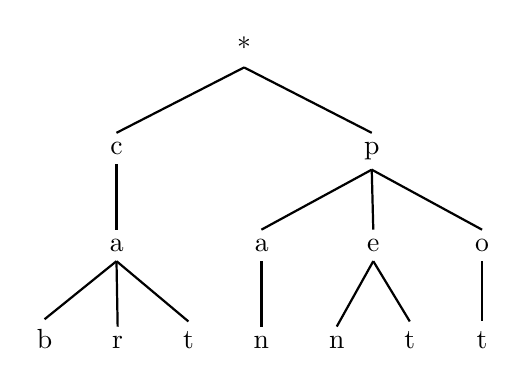
\begin{tikzpicture}
    \tikzset{level distance=3.5em, sibling distance=1.5em, edge from parent/.append style={thick} }
    \Tree [.* [.c [.a b r t ] ] [.p [.a n ] [.e n t ] [.o t ] ] ]
  \end{tikzpicture}
  \end{center}
}

\subsection{junit-quickcheck}
\frame{\frametitle{junit-quickcheck}
  \begin{itemize}
    \item Based on \texttt{org.junit.experimental.theories.*}
    \item Annotation-based
    \item On \href{https://github.com/pholser/junit-quickcheck}{github.com} by @pholser
    \item 0.3 version in maven repository
    \item Found \href{https://github.com/pholser/junit-quickcheck/issues/35}{bug with generics} during making presentation
  \end{itemize}
}

\frame{\frametitle{Demo}
  \begin{center}
    \includegraphics[height=0.8\textheight]{not_ready.jpg}
  \end{center}
}

\subsection{JCheck}
\frame{\frametitle{JCheck}
  \begin{itemize}
    \item Has its own JUnit Runner
    \item Annotation-based
    \item On \href{http://sourceforge.net/projects/jcheck/}{sf.net} by @hampusr
    \item 0.1 version jar from 2008
  \end{itemize}
}

\frame{\frametitle{Demo}
  \begin{center}
    \includegraphics[height=0.8\textheight]{show_code.jpg}
  \end{center}
}

\subsection{quickcheck}
\frame{\frametitle{quickcheck}
  \begin{itemize}
    \item Do not have Runner at all
    \item Handle only data generation
    \item On \href{https://bitbucket.org/blob79/quickcheck}{bitbucket.org} by @blob79
    \item 0.6 version in maven repository
  \end{itemize}
}

\frame{\frametitle{Demo}
  \begin{center}
    \includegraphics[height=0.8\textheight]{finally.jpeg} 
  \end{center}
}

\section{Where can we use it?}
\frame{\frametitle{ThinkScript}
  \begin{itemize}
    \item Programming language for traders
    \item Technical analisys
    \item Has a lot of built-in functions (SMA, EMA, WMA, ...)
  \end{itemize}
}

\frame{\frametitle{Standard deviation}
  \begin{center}
    \Large{$\sigma = \sqrt{\frac{1}{N} \sum_{i=1}^N (x_i - \mu)^2}$, \\
    $\mu = \frac{1}{N} \sum_{i=1}^N x_i$}
  \end{center}
}

\frame{\frametitle{Demo}
  \begin{center}
    \includegraphics[height=0.8\textheight]{we_can.png} 
  \end{center}
}

\frame{\frametitle{Donald Knuth is shocked by stdev}
  \begin{center}
    \includegraphics[width=0.8\textwidth]{knuth.png} 
  \end{center}
}

\frame{\frametitle{Where can we use it?}
  \begin{itemize}
    \item<1-> In Thinkscript, dxStudies - almost everywhere
    \item<2-> Regression tests - almost everywhere
    \item<3-> TosChart - configurations testing
    \item<4-> Often instead of regular xUnit
  \end{itemize}
}
% Ссылки 
\section{Links}
\frame{\frametitle{Links}
  \begin{itemize}
    \item \href{https://github.com/gark87/job-misc/tree/master/presentations/check_it_out/JohnDoeProject}{JohnDoeProject with examples} $\vcenter{\hbox{\includegraphics[width=2.5em]{github.png}}}$
    \item \href{http://www.haskell.org/haskellwiki/Introduction_to_QuickCheck2}{Introduction to QuickCheck2}
    \item \href{http://theyougen.blogspot.ru/search/label/quickcheck}{Blog dedicated to Java Quickcheck}
    \item \href{http://thinkrelevance.com/blog/2013/11/26/better-than-unit-tests}{Better Than Unit Tests}
  \end{itemize}
}
\frame{\frametitle{Thank you!}
  \begin{center}
    \includegraphics[height=0.8\textheight]{last.jpg}
  \end{center}
}

\end{document}
